
\documentclass{standalone}

%\documentclass[convert]{standalone}
% convert: in addition to pdf output files, png files are created
% convert options does work properly with -output-directory option of latexmk

\usepackage{tikz-feynman}
\tikzfeynmanset{compat=1.1.0}


\begin{document}
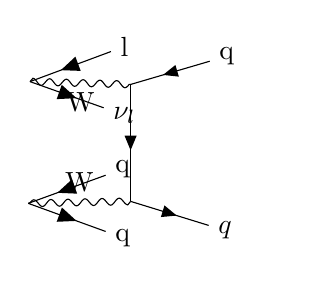
\begin{tikzpicture}
          \begin{feynman}
            \diagram [small, vertical=a to b] {
            % t-channel ttbar, qq -> gg -- > bbtt

            qi1 [particle=q] -- [fermion] a -- [boson, edge label=W] w,
            %qi2 [particle=q]  -- b -- [gluon, edge label=g] g2,
            w2 -- [boson, edge label=W] b -- [fermion] qi2 [particle=\( q \)] ,

            a -- [fermion] b,

            % invisible helper
            qi1 -- [draw=none] invis -- [draw=none] qi2,
            w -- [draw=none] w2,
            };

            \vertex [right=1.2cm of w] (b12_invis_helper);    % helper
            \vertex [above=0.2cm of b12_invis_helper] (b1) {l};
            \vertex [below=0.2cm of b12_invis_helper] (b2) {$\nu_{l}$};
            \draw [fermion] (b1) -- (w);
            \draw [fermion] (w) -- (b2);

            \vertex [right=1.2cm of w2] (t12_invis_helper);    % helper
            \vertex [above=0.2cm of t12_invis_helper] (qo1) {q};
            \vertex [below=0.2cm of t12_invis_helper] (qo2) {q};
            \draw [fermion] (qo1) -- (w2);
            \draw [fermion] (w2) -- (qo2);
          \end{feynman}
        \end{tikzpicture}
\end{document}
